%
% db1.tex -- daubechies wavelet 1
%
% (c) 2019 Prof Dr Andreas Müller, Hochschule Rapperswil
%
\documentclass[tikz]{standalone}
\usepackage{amsmath}
\usepackage{times}
\usepackage{txfonts}
\usepackage{pgfplots}
\usepackage{csvsimple}
\usetikzlibrary{arrows,intersections,math}
\begin{document}
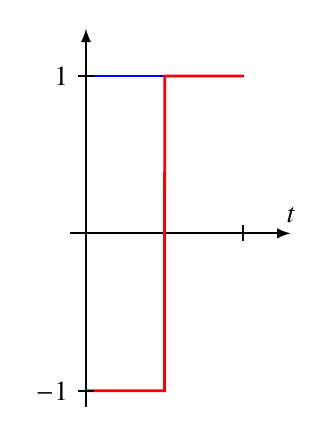
\begin{tikzpicture}[>=latex,scale=2]

\draw[->,line width=0.7pt] (-0.1,0)--(1.3,0) coordinate[label={$t$}];
\draw[->,line width=0.7pt] (0,-1.1)--(0,1.3);

\draw[line width=1pt,color=blue] (0.00000, 1.00000)
--(0.00195, 1.00000)
--(0.00391, 1.00000)
--(0.00586, 1.00000)
--(0.00781, 1.00000)
--(0.00977, 1.00000)
--(0.01172, 1.00000)
--(0.01367, 1.00000)
--(0.01562, 1.00000)
--(0.01758, 1.00000)
--(0.01953, 1.00000)
--(0.02148, 1.00000)
--(0.02344, 1.00000)
--(0.02539, 1.00000)
--(0.02734, 1.00000)
--(0.02930, 1.00000)
--(0.03125, 1.00000)
--(0.03320, 1.00000)
--(0.03516, 1.00000)
--(0.03711, 1.00000)
--(0.03906, 1.00000)
--(0.04102, 1.00000)
--(0.04297, 1.00000)
--(0.04492, 1.00000)
--(0.04688, 1.00000)
--(0.04883, 1.00000)
--(0.05078, 1.00000)
--(0.05273, 1.00000)
--(0.05469, 1.00000)
--(0.05664, 1.00000)
--(0.05859, 1.00000)
--(0.06055, 1.00000)
--(0.06250, 1.00000)
--(0.06445, 1.00000)
--(0.06641, 1.00000)
--(0.06836, 1.00000)
--(0.07031, 1.00000)
--(0.07227, 1.00000)
--(0.07422, 1.00000)
--(0.07617, 1.00000)
--(0.07812, 1.00000)
--(0.08008, 1.00000)
--(0.08203, 1.00000)
--(0.08398, 1.00000)
--(0.08594, 1.00000)
--(0.08789, 1.00000)
--(0.08984, 1.00000)
--(0.09180, 1.00000)
--(0.09375, 1.00000)
--(0.09570, 1.00000)
--(0.09766, 1.00000)
--(0.09961, 1.00000)
--(0.10156, 1.00000)
--(0.10352, 1.00000)
--(0.10547, 1.00000)
--(0.10742, 1.00000)
--(0.10938, 1.00000)
--(0.11133, 1.00000)
--(0.11328, 1.00000)
--(0.11523, 1.00000)
--(0.11719, 1.00000)
--(0.11914, 1.00000)
--(0.12109, 1.00000)
--(0.12305, 1.00000)
--(0.12500, 1.00000)
--(0.12695, 1.00000)
--(0.12891, 1.00000)
--(0.13086, 1.00000)
--(0.13281, 1.00000)
--(0.13477, 1.00000)
--(0.13672, 1.00000)
--(0.13867, 1.00000)
--(0.14062, 1.00000)
--(0.14258, 1.00000)
--(0.14453, 1.00000)
--(0.14648, 1.00000)
--(0.14844, 1.00000)
--(0.15039, 1.00000)
--(0.15234, 1.00000)
--(0.15430, 1.00000)
--(0.15625, 1.00000)
--(0.15820, 1.00000)
--(0.16016, 1.00000)
--(0.16211, 1.00000)
--(0.16406, 1.00000)
--(0.16602, 1.00000)
--(0.16797, 1.00000)
--(0.16992, 1.00000)
--(0.17188, 1.00000)
--(0.17383, 1.00000)
--(0.17578, 1.00000)
--(0.17773, 1.00000)
--(0.17969, 1.00000)
--(0.18164, 1.00000)
--(0.18359, 1.00000)
--(0.18555, 1.00000)
--(0.18750, 1.00000)
--(0.18945, 1.00000)
--(0.19141, 1.00000)
--(0.19336, 1.00000)
--(0.19531, 1.00000)
--(0.19727, 1.00000)
--(0.19922, 1.00000)
--(0.20117, 1.00000)
--(0.20312, 1.00000)
--(0.20508, 1.00000)
--(0.20703, 1.00000)
--(0.20898, 1.00000)
--(0.21094, 1.00000)
--(0.21289, 1.00000)
--(0.21484, 1.00000)
--(0.21680, 1.00000)
--(0.21875, 1.00000)
--(0.22070, 1.00000)
--(0.22266, 1.00000)
--(0.22461, 1.00000)
--(0.22656, 1.00000)
--(0.22852, 1.00000)
--(0.23047, 1.00000)
--(0.23242, 1.00000)
--(0.23438, 1.00000)
--(0.23633, 1.00000)
--(0.23828, 1.00000)
--(0.24023, 1.00000)
--(0.24219, 1.00000)
--(0.24414, 1.00000)
--(0.24609, 1.00000)
--(0.24805, 1.00000)
--(0.25000, 1.00000)
--(0.25195, 1.00000)
--(0.25391, 1.00000)
--(0.25586, 1.00000)
--(0.25781, 1.00000)
--(0.25977, 1.00000)
--(0.26172, 1.00000)
--(0.26367, 1.00000)
--(0.26562, 1.00000)
--(0.26758, 1.00000)
--(0.26953, 1.00000)
--(0.27148, 1.00000)
--(0.27344, 1.00000)
--(0.27539, 1.00000)
--(0.27734, 1.00000)
--(0.27930, 1.00000)
--(0.28125, 1.00000)
--(0.28320, 1.00000)
--(0.28516, 1.00000)
--(0.28711, 1.00000)
--(0.28906, 1.00000)
--(0.29102, 1.00000)
--(0.29297, 1.00000)
--(0.29492, 1.00000)
--(0.29688, 1.00000)
--(0.29883, 1.00000)
--(0.30078, 1.00000)
--(0.30273, 1.00000)
--(0.30469, 1.00000)
--(0.30664, 1.00000)
--(0.30859, 1.00000)
--(0.31055, 1.00000)
--(0.31250, 1.00000)
--(0.31445, 1.00000)
--(0.31641, 1.00000)
--(0.31836, 1.00000)
--(0.32031, 1.00000)
--(0.32227, 1.00000)
--(0.32422, 1.00000)
--(0.32617, 1.00000)
--(0.32812, 1.00000)
--(0.33008, 1.00000)
--(0.33203, 1.00000)
--(0.33398, 1.00000)
--(0.33594, 1.00000)
--(0.33789, 1.00000)
--(0.33984, 1.00000)
--(0.34180, 1.00000)
--(0.34375, 1.00000)
--(0.34570, 1.00000)
--(0.34766, 1.00000)
--(0.34961, 1.00000)
--(0.35156, 1.00000)
--(0.35352, 1.00000)
--(0.35547, 1.00000)
--(0.35742, 1.00000)
--(0.35938, 1.00000)
--(0.36133, 1.00000)
--(0.36328, 1.00000)
--(0.36523, 1.00000)
--(0.36719, 1.00000)
--(0.36914, 1.00000)
--(0.37109, 1.00000)
--(0.37305, 1.00000)
--(0.37500, 1.00000)
--(0.37695, 1.00000)
--(0.37891, 1.00000)
--(0.38086, 1.00000)
--(0.38281, 1.00000)
--(0.38477, 1.00000)
--(0.38672, 1.00000)
--(0.38867, 1.00000)
--(0.39062, 1.00000)
--(0.39258, 1.00000)
--(0.39453, 1.00000)
--(0.39648, 1.00000)
--(0.39844, 1.00000)
--(0.40039, 1.00000)
--(0.40234, 1.00000)
--(0.40430, 1.00000)
--(0.40625, 1.00000)
--(0.40820, 1.00000)
--(0.41016, 1.00000)
--(0.41211, 1.00000)
--(0.41406, 1.00000)
--(0.41602, 1.00000)
--(0.41797, 1.00000)
--(0.41992, 1.00000)
--(0.42188, 1.00000)
--(0.42383, 1.00000)
--(0.42578, 1.00000)
--(0.42773, 1.00000)
--(0.42969, 1.00000)
--(0.43164, 1.00000)
--(0.43359, 1.00000)
--(0.43555, 1.00000)
--(0.43750, 1.00000)
--(0.43945, 1.00000)
--(0.44141, 1.00000)
--(0.44336, 1.00000)
--(0.44531, 1.00000)
--(0.44727, 1.00000)
--(0.44922, 1.00000)
--(0.45117, 1.00000)
--(0.45312, 1.00000)
--(0.45508, 1.00000)
--(0.45703, 1.00000)
--(0.45898, 1.00000)
--(0.46094, 1.00000)
--(0.46289, 1.00000)
--(0.46484, 1.00000)
--(0.46680, 1.00000)
--(0.46875, 1.00000)
--(0.47070, 1.00000)
--(0.47266, 1.00000)
--(0.47461, 1.00000)
--(0.47656, 1.00000)
--(0.47852, 1.00000)
--(0.48047, 1.00000)
--(0.48242, 1.00000)
--(0.48438, 1.00000)
--(0.48633, 1.00000)
--(0.48828, 1.00000)
--(0.49023, 1.00000)
--(0.49219, 1.00000)
--(0.49414, 1.00000)
--(0.49609, 1.00000)
--(0.49805, 1.00000)
--(0.50000, 1.00000)
--(0.50195, 1.00000)
--(0.50391, 1.00000)
--(0.50586, 1.00000)
--(0.50781, 1.00000)
--(0.50977, 1.00000)
--(0.51172, 1.00000)
--(0.51367, 1.00000)
--(0.51562, 1.00000)
--(0.51758, 1.00000)
--(0.51953, 1.00000)
--(0.52148, 1.00000)
--(0.52344, 1.00000)
--(0.52539, 1.00000)
--(0.52734, 1.00000)
--(0.52930, 1.00000)
--(0.53125, 1.00000)
--(0.53320, 1.00000)
--(0.53516, 1.00000)
--(0.53711, 1.00000)
--(0.53906, 1.00000)
--(0.54102, 1.00000)
--(0.54297, 1.00000)
--(0.54492, 1.00000)
--(0.54688, 1.00000)
--(0.54883, 1.00000)
--(0.55078, 1.00000)
--(0.55273, 1.00000)
--(0.55469, 1.00000)
--(0.55664, 1.00000)
--(0.55859, 1.00000)
--(0.56055, 1.00000)
--(0.56250, 1.00000)
--(0.56445, 1.00000)
--(0.56641, 1.00000)
--(0.56836, 1.00000)
--(0.57031, 1.00000)
--(0.57227, 1.00000)
--(0.57422, 1.00000)
--(0.57617, 1.00000)
--(0.57812, 1.00000)
--(0.58008, 1.00000)
--(0.58203, 1.00000)
--(0.58398, 1.00000)
--(0.58594, 1.00000)
--(0.58789, 1.00000)
--(0.58984, 1.00000)
--(0.59180, 1.00000)
--(0.59375, 1.00000)
--(0.59570, 1.00000)
--(0.59766, 1.00000)
--(0.59961, 1.00000)
--(0.60156, 1.00000)
--(0.60352, 1.00000)
--(0.60547, 1.00000)
--(0.60742, 1.00000)
--(0.60938, 1.00000)
--(0.61133, 1.00000)
--(0.61328, 1.00000)
--(0.61523, 1.00000)
--(0.61719, 1.00000)
--(0.61914, 1.00000)
--(0.62109, 1.00000)
--(0.62305, 1.00000)
--(0.62500, 1.00000)
--(0.62695, 1.00000)
--(0.62891, 1.00000)
--(0.63086, 1.00000)
--(0.63281, 1.00000)
--(0.63477, 1.00000)
--(0.63672, 1.00000)
--(0.63867, 1.00000)
--(0.64062, 1.00000)
--(0.64258, 1.00000)
--(0.64453, 1.00000)
--(0.64648, 1.00000)
--(0.64844, 1.00000)
--(0.65039, 1.00000)
--(0.65234, 1.00000)
--(0.65430, 1.00000)
--(0.65625, 1.00000)
--(0.65820, 1.00000)
--(0.66016, 1.00000)
--(0.66211, 1.00000)
--(0.66406, 1.00000)
--(0.66602, 1.00000)
--(0.66797, 1.00000)
--(0.66992, 1.00000)
--(0.67188, 1.00000)
--(0.67383, 1.00000)
--(0.67578, 1.00000)
--(0.67773, 1.00000)
--(0.67969, 1.00000)
--(0.68164, 1.00000)
--(0.68359, 1.00000)
--(0.68555, 1.00000)
--(0.68750, 1.00000)
--(0.68945, 1.00000)
--(0.69141, 1.00000)
--(0.69336, 1.00000)
--(0.69531, 1.00000)
--(0.69727, 1.00000)
--(0.69922, 1.00000)
--(0.70117, 1.00000)
--(0.70312, 1.00000)
--(0.70508, 1.00000)
--(0.70703, 1.00000)
--(0.70898, 1.00000)
--(0.71094, 1.00000)
--(0.71289, 1.00000)
--(0.71484, 1.00000)
--(0.71680, 1.00000)
--(0.71875, 1.00000)
--(0.72070, 1.00000)
--(0.72266, 1.00000)
--(0.72461, 1.00000)
--(0.72656, 1.00000)
--(0.72852, 1.00000)
--(0.73047, 1.00000)
--(0.73242, 1.00000)
--(0.73438, 1.00000)
--(0.73633, 1.00000)
--(0.73828, 1.00000)
--(0.74023, 1.00000)
--(0.74219, 1.00000)
--(0.74414, 1.00000)
--(0.74609, 1.00000)
--(0.74805, 1.00000)
--(0.75000, 1.00000)
--(0.75195, 1.00000)
--(0.75391, 1.00000)
--(0.75586, 1.00000)
--(0.75781, 1.00000)
--(0.75977, 1.00000)
--(0.76172, 1.00000)
--(0.76367, 1.00000)
--(0.76562, 1.00000)
--(0.76758, 1.00000)
--(0.76953, 1.00000)
--(0.77148, 1.00000)
--(0.77344, 1.00000)
--(0.77539, 1.00000)
--(0.77734, 1.00000)
--(0.77930, 1.00000)
--(0.78125, 1.00000)
--(0.78320, 1.00000)
--(0.78516, 1.00000)
--(0.78711, 1.00000)
--(0.78906, 1.00000)
--(0.79102, 1.00000)
--(0.79297, 1.00000)
--(0.79492, 1.00000)
--(0.79688, 1.00000)
--(0.79883, 1.00000)
--(0.80078, 1.00000)
--(0.80273, 1.00000)
--(0.80469, 1.00000)
--(0.80664, 1.00000)
--(0.80859, 1.00000)
--(0.81055, 1.00000)
--(0.81250, 1.00000)
--(0.81445, 1.00000)
--(0.81641, 1.00000)
--(0.81836, 1.00000)
--(0.82031, 1.00000)
--(0.82227, 1.00000)
--(0.82422, 1.00000)
--(0.82617, 1.00000)
--(0.82812, 1.00000)
--(0.83008, 1.00000)
--(0.83203, 1.00000)
--(0.83398, 1.00000)
--(0.83594, 1.00000)
--(0.83789, 1.00000)
--(0.83984, 1.00000)
--(0.84180, 1.00000)
--(0.84375, 1.00000)
--(0.84570, 1.00000)
--(0.84766, 1.00000)
--(0.84961, 1.00000)
--(0.85156, 1.00000)
--(0.85352, 1.00000)
--(0.85547, 1.00000)
--(0.85742, 1.00000)
--(0.85938, 1.00000)
--(0.86133, 1.00000)
--(0.86328, 1.00000)
--(0.86523, 1.00000)
--(0.86719, 1.00000)
--(0.86914, 1.00000)
--(0.87109, 1.00000)
--(0.87305, 1.00000)
--(0.87500, 1.00000)
--(0.87695, 1.00000)
--(0.87891, 1.00000)
--(0.88086, 1.00000)
--(0.88281, 1.00000)
--(0.88477, 1.00000)
--(0.88672, 1.00000)
--(0.88867, 1.00000)
--(0.89062, 1.00000)
--(0.89258, 1.00000)
--(0.89453, 1.00000)
--(0.89648, 1.00000)
--(0.89844, 1.00000)
--(0.90039, 1.00000)
--(0.90234, 1.00000)
--(0.90430, 1.00000)
--(0.90625, 1.00000)
--(0.90820, 1.00000)
--(0.91016, 1.00000)
--(0.91211, 1.00000)
--(0.91406, 1.00000)
--(0.91602, 1.00000)
--(0.91797, 1.00000)
--(0.91992, 1.00000)
--(0.92188, 1.00000)
--(0.92383, 1.00000)
--(0.92578, 1.00000)
--(0.92773, 1.00000)
--(0.92969, 1.00000)
--(0.93164, 1.00000)
--(0.93359, 1.00000)
--(0.93555, 1.00000)
--(0.93750, 1.00000)
--(0.93945, 1.00000)
--(0.94141, 1.00000)
--(0.94336, 1.00000)
--(0.94531, 1.00000)
--(0.94727, 1.00000)
--(0.94922, 1.00000)
--(0.95117, 1.00000)
--(0.95312, 1.00000)
--(0.95508, 1.00000)
--(0.95703, 1.00000)
--(0.95898, 1.00000)
--(0.96094, 1.00000)
--(0.96289, 1.00000)
--(0.96484, 1.00000)
--(0.96680, 1.00000)
--(0.96875, 1.00000)
--(0.97070, 1.00000)
--(0.97266, 1.00000)
--(0.97461, 1.00000)
--(0.97656, 1.00000)
--(0.97852, 1.00000)
--(0.98047, 1.00000)
--(0.98242, 1.00000)
--(0.98438, 1.00000)
--(0.98633, 1.00000)
--(0.98828, 1.00000)
--(0.99023, 1.00000)
--(0.99219, 1.00000)
--(0.99414, 1.00000)
--(0.99609, 1.00000)
--(0.99805, 1.00000)
;

\draw[line width=1pt,color=red] (0.00000, -1.00000)
--(0.00195, -1.00000)
--(0.00391, -1.00000)
--(0.00586, -1.00000)
--(0.00781, -1.00000)
--(0.00977, -1.00000)
--(0.01172, -1.00000)
--(0.01367, -1.00000)
--(0.01562, -1.00000)
--(0.01758, -1.00000)
--(0.01953, -1.00000)
--(0.02148, -1.00000)
--(0.02344, -1.00000)
--(0.02539, -1.00000)
--(0.02734, -1.00000)
--(0.02930, -1.00000)
--(0.03125, -1.00000)
--(0.03320, -1.00000)
--(0.03516, -1.00000)
--(0.03711, -1.00000)
--(0.03906, -1.00000)
--(0.04102, -1.00000)
--(0.04297, -1.00000)
--(0.04492, -1.00000)
--(0.04688, -1.00000)
--(0.04883, -1.00000)
--(0.05078, -1.00000)
--(0.05273, -1.00000)
--(0.05469, -1.00000)
--(0.05664, -1.00000)
--(0.05859, -1.00000)
--(0.06055, -1.00000)
--(0.06250, -1.00000)
--(0.06445, -1.00000)
--(0.06641, -1.00000)
--(0.06836, -1.00000)
--(0.07031, -1.00000)
--(0.07227, -1.00000)
--(0.07422, -1.00000)
--(0.07617, -1.00000)
--(0.07812, -1.00000)
--(0.08008, -1.00000)
--(0.08203, -1.00000)
--(0.08398, -1.00000)
--(0.08594, -1.00000)
--(0.08789, -1.00000)
--(0.08984, -1.00000)
--(0.09180, -1.00000)
--(0.09375, -1.00000)
--(0.09570, -1.00000)
--(0.09766, -1.00000)
--(0.09961, -1.00000)
--(0.10156, -1.00000)
--(0.10352, -1.00000)
--(0.10547, -1.00000)
--(0.10742, -1.00000)
--(0.10938, -1.00000)
--(0.11133, -1.00000)
--(0.11328, -1.00000)
--(0.11523, -1.00000)
--(0.11719, -1.00000)
--(0.11914, -1.00000)
--(0.12109, -1.00000)
--(0.12305, -1.00000)
--(0.12500, -1.00000)
--(0.12695, -1.00000)
--(0.12891, -1.00000)
--(0.13086, -1.00000)
--(0.13281, -1.00000)
--(0.13477, -1.00000)
--(0.13672, -1.00000)
--(0.13867, -1.00000)
--(0.14062, -1.00000)
--(0.14258, -1.00000)
--(0.14453, -1.00000)
--(0.14648, -1.00000)
--(0.14844, -1.00000)
--(0.15039, -1.00000)
--(0.15234, -1.00000)
--(0.15430, -1.00000)
--(0.15625, -1.00000)
--(0.15820, -1.00000)
--(0.16016, -1.00000)
--(0.16211, -1.00000)
--(0.16406, -1.00000)
--(0.16602, -1.00000)
--(0.16797, -1.00000)
--(0.16992, -1.00000)
--(0.17188, -1.00000)
--(0.17383, -1.00000)
--(0.17578, -1.00000)
--(0.17773, -1.00000)
--(0.17969, -1.00000)
--(0.18164, -1.00000)
--(0.18359, -1.00000)
--(0.18555, -1.00000)
--(0.18750, -1.00000)
--(0.18945, -1.00000)
--(0.19141, -1.00000)
--(0.19336, -1.00000)
--(0.19531, -1.00000)
--(0.19727, -1.00000)
--(0.19922, -1.00000)
--(0.20117, -1.00000)
--(0.20312, -1.00000)
--(0.20508, -1.00000)
--(0.20703, -1.00000)
--(0.20898, -1.00000)
--(0.21094, -1.00000)
--(0.21289, -1.00000)
--(0.21484, -1.00000)
--(0.21680, -1.00000)
--(0.21875, -1.00000)
--(0.22070, -1.00000)
--(0.22266, -1.00000)
--(0.22461, -1.00000)
--(0.22656, -1.00000)
--(0.22852, -1.00000)
--(0.23047, -1.00000)
--(0.23242, -1.00000)
--(0.23438, -1.00000)
--(0.23633, -1.00000)
--(0.23828, -1.00000)
--(0.24023, -1.00000)
--(0.24219, -1.00000)
--(0.24414, -1.00000)
--(0.24609, -1.00000)
--(0.24805, -1.00000)
--(0.25000, -1.00000)
--(0.25195, -1.00000)
--(0.25391, -1.00000)
--(0.25586, -1.00000)
--(0.25781, -1.00000)
--(0.25977, -1.00000)
--(0.26172, -1.00000)
--(0.26367, -1.00000)
--(0.26562, -1.00000)
--(0.26758, -1.00000)
--(0.26953, -1.00000)
--(0.27148, -1.00000)
--(0.27344, -1.00000)
--(0.27539, -1.00000)
--(0.27734, -1.00000)
--(0.27930, -1.00000)
--(0.28125, -1.00000)
--(0.28320, -1.00000)
--(0.28516, -1.00000)
--(0.28711, -1.00000)
--(0.28906, -1.00000)
--(0.29102, -1.00000)
--(0.29297, -1.00000)
--(0.29492, -1.00000)
--(0.29688, -1.00000)
--(0.29883, -1.00000)
--(0.30078, -1.00000)
--(0.30273, -1.00000)
--(0.30469, -1.00000)
--(0.30664, -1.00000)
--(0.30859, -1.00000)
--(0.31055, -1.00000)
--(0.31250, -1.00000)
--(0.31445, -1.00000)
--(0.31641, -1.00000)
--(0.31836, -1.00000)
--(0.32031, -1.00000)
--(0.32227, -1.00000)
--(0.32422, -1.00000)
--(0.32617, -1.00000)
--(0.32812, -1.00000)
--(0.33008, -1.00000)
--(0.33203, -1.00000)
--(0.33398, -1.00000)
--(0.33594, -1.00000)
--(0.33789, -1.00000)
--(0.33984, -1.00000)
--(0.34180, -1.00000)
--(0.34375, -1.00000)
--(0.34570, -1.00000)
--(0.34766, -1.00000)
--(0.34961, -1.00000)
--(0.35156, -1.00000)
--(0.35352, -1.00000)
--(0.35547, -1.00000)
--(0.35742, -1.00000)
--(0.35938, -1.00000)
--(0.36133, -1.00000)
--(0.36328, -1.00000)
--(0.36523, -1.00000)
--(0.36719, -1.00000)
--(0.36914, -1.00000)
--(0.37109, -1.00000)
--(0.37305, -1.00000)
--(0.37500, -1.00000)
--(0.37695, -1.00000)
--(0.37891, -1.00000)
--(0.38086, -1.00000)
--(0.38281, -1.00000)
--(0.38477, -1.00000)
--(0.38672, -1.00000)
--(0.38867, -1.00000)
--(0.39062, -1.00000)
--(0.39258, -1.00000)
--(0.39453, -1.00000)
--(0.39648, -1.00000)
--(0.39844, -1.00000)
--(0.40039, -1.00000)
--(0.40234, -1.00000)
--(0.40430, -1.00000)
--(0.40625, -1.00000)
--(0.40820, -1.00000)
--(0.41016, -1.00000)
--(0.41211, -1.00000)
--(0.41406, -1.00000)
--(0.41602, -1.00000)
--(0.41797, -1.00000)
--(0.41992, -1.00000)
--(0.42188, -1.00000)
--(0.42383, -1.00000)
--(0.42578, -1.00000)
--(0.42773, -1.00000)
--(0.42969, -1.00000)
--(0.43164, -1.00000)
--(0.43359, -1.00000)
--(0.43555, -1.00000)
--(0.43750, -1.00000)
--(0.43945, -1.00000)
--(0.44141, -1.00000)
--(0.44336, -1.00000)
--(0.44531, -1.00000)
--(0.44727, -1.00000)
--(0.44922, -1.00000)
--(0.45117, -1.00000)
--(0.45312, -1.00000)
--(0.45508, -1.00000)
--(0.45703, -1.00000)
--(0.45898, -1.00000)
--(0.46094, -1.00000)
--(0.46289, -1.00000)
--(0.46484, -1.00000)
--(0.46680, -1.00000)
--(0.46875, -1.00000)
--(0.47070, -1.00000)
--(0.47266, -1.00000)
--(0.47461, -1.00000)
--(0.47656, -1.00000)
--(0.47852, -1.00000)
--(0.48047, -1.00000)
--(0.48242, -1.00000)
--(0.48438, -1.00000)
--(0.48633, -1.00000)
--(0.48828, -1.00000)
--(0.49023, -1.00000)
--(0.49219, -1.00000)
--(0.49414, -1.00000)
--(0.49609, -1.00000)
--(0.49805, -1.00000)
--(0.50000, 1.00000)
--(0.50195, 1.00000)
--(0.50391, 1.00000)
--(0.50586, 1.00000)
--(0.50781, 1.00000)
--(0.50977, 1.00000)
--(0.51172, 1.00000)
--(0.51367, 1.00000)
--(0.51562, 1.00000)
--(0.51758, 1.00000)
--(0.51953, 1.00000)
--(0.52148, 1.00000)
--(0.52344, 1.00000)
--(0.52539, 1.00000)
--(0.52734, 1.00000)
--(0.52930, 1.00000)
--(0.53125, 1.00000)
--(0.53320, 1.00000)
--(0.53516, 1.00000)
--(0.53711, 1.00000)
--(0.53906, 1.00000)
--(0.54102, 1.00000)
--(0.54297, 1.00000)
--(0.54492, 1.00000)
--(0.54688, 1.00000)
--(0.54883, 1.00000)
--(0.55078, 1.00000)
--(0.55273, 1.00000)
--(0.55469, 1.00000)
--(0.55664, 1.00000)
--(0.55859, 1.00000)
--(0.56055, 1.00000)
--(0.56250, 1.00000)
--(0.56445, 1.00000)
--(0.56641, 1.00000)
--(0.56836, 1.00000)
--(0.57031, 1.00000)
--(0.57227, 1.00000)
--(0.57422, 1.00000)
--(0.57617, 1.00000)
--(0.57812, 1.00000)
--(0.58008, 1.00000)
--(0.58203, 1.00000)
--(0.58398, 1.00000)
--(0.58594, 1.00000)
--(0.58789, 1.00000)
--(0.58984, 1.00000)
--(0.59180, 1.00000)
--(0.59375, 1.00000)
--(0.59570, 1.00000)
--(0.59766, 1.00000)
--(0.59961, 1.00000)
--(0.60156, 1.00000)
--(0.60352, 1.00000)
--(0.60547, 1.00000)
--(0.60742, 1.00000)
--(0.60938, 1.00000)
--(0.61133, 1.00000)
--(0.61328, 1.00000)
--(0.61523, 1.00000)
--(0.61719, 1.00000)
--(0.61914, 1.00000)
--(0.62109, 1.00000)
--(0.62305, 1.00000)
--(0.62500, 1.00000)
--(0.62695, 1.00000)
--(0.62891, 1.00000)
--(0.63086, 1.00000)
--(0.63281, 1.00000)
--(0.63477, 1.00000)
--(0.63672, 1.00000)
--(0.63867, 1.00000)
--(0.64062, 1.00000)
--(0.64258, 1.00000)
--(0.64453, 1.00000)
--(0.64648, 1.00000)
--(0.64844, 1.00000)
--(0.65039, 1.00000)
--(0.65234, 1.00000)
--(0.65430, 1.00000)
--(0.65625, 1.00000)
--(0.65820, 1.00000)
--(0.66016, 1.00000)
--(0.66211, 1.00000)
--(0.66406, 1.00000)
--(0.66602, 1.00000)
--(0.66797, 1.00000)
--(0.66992, 1.00000)
--(0.67188, 1.00000)
--(0.67383, 1.00000)
--(0.67578, 1.00000)
--(0.67773, 1.00000)
--(0.67969, 1.00000)
--(0.68164, 1.00000)
--(0.68359, 1.00000)
--(0.68555, 1.00000)
--(0.68750, 1.00000)
--(0.68945, 1.00000)
--(0.69141, 1.00000)
--(0.69336, 1.00000)
--(0.69531, 1.00000)
--(0.69727, 1.00000)
--(0.69922, 1.00000)
--(0.70117, 1.00000)
--(0.70312, 1.00000)
--(0.70508, 1.00000)
--(0.70703, 1.00000)
--(0.70898, 1.00000)
--(0.71094, 1.00000)
--(0.71289, 1.00000)
--(0.71484, 1.00000)
--(0.71680, 1.00000)
--(0.71875, 1.00000)
--(0.72070, 1.00000)
--(0.72266, 1.00000)
--(0.72461, 1.00000)
--(0.72656, 1.00000)
--(0.72852, 1.00000)
--(0.73047, 1.00000)
--(0.73242, 1.00000)
--(0.73438, 1.00000)
--(0.73633, 1.00000)
--(0.73828, 1.00000)
--(0.74023, 1.00000)
--(0.74219, 1.00000)
--(0.74414, 1.00000)
--(0.74609, 1.00000)
--(0.74805, 1.00000)
--(0.75000, 1.00000)
--(0.75195, 1.00000)
--(0.75391, 1.00000)
--(0.75586, 1.00000)
--(0.75781, 1.00000)
--(0.75977, 1.00000)
--(0.76172, 1.00000)
--(0.76367, 1.00000)
--(0.76562, 1.00000)
--(0.76758, 1.00000)
--(0.76953, 1.00000)
--(0.77148, 1.00000)
--(0.77344, 1.00000)
--(0.77539, 1.00000)
--(0.77734, 1.00000)
--(0.77930, 1.00000)
--(0.78125, 1.00000)
--(0.78320, 1.00000)
--(0.78516, 1.00000)
--(0.78711, 1.00000)
--(0.78906, 1.00000)
--(0.79102, 1.00000)
--(0.79297, 1.00000)
--(0.79492, 1.00000)
--(0.79688, 1.00000)
--(0.79883, 1.00000)
--(0.80078, 1.00000)
--(0.80273, 1.00000)
--(0.80469, 1.00000)
--(0.80664, 1.00000)
--(0.80859, 1.00000)
--(0.81055, 1.00000)
--(0.81250, 1.00000)
--(0.81445, 1.00000)
--(0.81641, 1.00000)
--(0.81836, 1.00000)
--(0.82031, 1.00000)
--(0.82227, 1.00000)
--(0.82422, 1.00000)
--(0.82617, 1.00000)
--(0.82812, 1.00000)
--(0.83008, 1.00000)
--(0.83203, 1.00000)
--(0.83398, 1.00000)
--(0.83594, 1.00000)
--(0.83789, 1.00000)
--(0.83984, 1.00000)
--(0.84180, 1.00000)
--(0.84375, 1.00000)
--(0.84570, 1.00000)
--(0.84766, 1.00000)
--(0.84961, 1.00000)
--(0.85156, 1.00000)
--(0.85352, 1.00000)
--(0.85547, 1.00000)
--(0.85742, 1.00000)
--(0.85938, 1.00000)
--(0.86133, 1.00000)
--(0.86328, 1.00000)
--(0.86523, 1.00000)
--(0.86719, 1.00000)
--(0.86914, 1.00000)
--(0.87109, 1.00000)
--(0.87305, 1.00000)
--(0.87500, 1.00000)
--(0.87695, 1.00000)
--(0.87891, 1.00000)
--(0.88086, 1.00000)
--(0.88281, 1.00000)
--(0.88477, 1.00000)
--(0.88672, 1.00000)
--(0.88867, 1.00000)
--(0.89062, 1.00000)
--(0.89258, 1.00000)
--(0.89453, 1.00000)
--(0.89648, 1.00000)
--(0.89844, 1.00000)
--(0.90039, 1.00000)
--(0.90234, 1.00000)
--(0.90430, 1.00000)
--(0.90625, 1.00000)
--(0.90820, 1.00000)
--(0.91016, 1.00000)
--(0.91211, 1.00000)
--(0.91406, 1.00000)
--(0.91602, 1.00000)
--(0.91797, 1.00000)
--(0.91992, 1.00000)
--(0.92188, 1.00000)
--(0.92383, 1.00000)
--(0.92578, 1.00000)
--(0.92773, 1.00000)
--(0.92969, 1.00000)
--(0.93164, 1.00000)
--(0.93359, 1.00000)
--(0.93555, 1.00000)
--(0.93750, 1.00000)
--(0.93945, 1.00000)
--(0.94141, 1.00000)
--(0.94336, 1.00000)
--(0.94531, 1.00000)
--(0.94727, 1.00000)
--(0.94922, 1.00000)
--(0.95117, 1.00000)
--(0.95312, 1.00000)
--(0.95508, 1.00000)
--(0.95703, 1.00000)
--(0.95898, 1.00000)
--(0.96094, 1.00000)
--(0.96289, 1.00000)
--(0.96484, 1.00000)
--(0.96680, 1.00000)
--(0.96875, 1.00000)
--(0.97070, 1.00000)
--(0.97266, 1.00000)
--(0.97461, 1.00000)
--(0.97656, 1.00000)
--(0.97852, 1.00000)
--(0.98047, 1.00000)
--(0.98242, 1.00000)
--(0.98438, 1.00000)
--(0.98633, 1.00000)
--(0.98828, 1.00000)
--(0.99023, 1.00000)
--(0.99219, 1.00000)
--(0.99414, 1.00000)
--(0.99609, 1.00000)
--(0.99805, 1.00000)
;


\foreach \x in {1,...,1}{
	\draw[line width=0.7pt] ({\x},-0.05)--({\x},0.05);
}

\draw[line width=0.7pt] (-0.05,1)--(0.05,1);
\draw[line width=0.7pt] (-0.05,-1)--(0.05,-1);
\node at (-0.05,1) [left] {$1$};
\node at (-0.05,-1) [left] {$-1$};

\end{tikzpicture}
\end{document}
